\newcommand{\CLASSINPUTtoptextmargin}{2.4cm}
\newcommand{\CLASSINPUTbottomtextmargin}{4.6cm}
\documentclass[10pt,journal]{IEEEtran}%change to article
\usepackage[margin=1in]{geometry}
\usepackage[utf8]{inputenc}
\IEEEoverridecommandlockouts
\usepackage{cite}
\usepackage{ragged2e}
\usepackage{amsmath,amssymb,amsfonts}
\usepackage{algorithmic}
\usepackage{graphicx} % Required for inserting images
\usepackage{soul,color}
\usepackage{textcomp}
\usepackage{url,setspace}
\usepackage{amssymb}
\usepackage{booktabs} % For better table formatting
%\usepackage{siunitx}
%\usepackage{orcidlink}
\usepackage{multirow}
\usepackage{pgfplots}
\pgfplotsset{compat=1.17}
\usepackage{caption}
 \captionsetup{size=footnotesize,
    %justification=centering, %% not needed
    skip=5pt, position = bottom}
\graphicspath{ {./images/} }
\def\BibTeX{{\rm B\kern-.05em{\sc i\kern-.025em b}\kern-.08em
    T\kern-.1667em\lower.7ex\hbox{E}\kern-.125emX}}

\usepackage{tikz}
\usetikzlibrary{positioning, shapes.geometric}
\DeclareRobustCommand{\hlcyan}[1]{{\sethlcolor{cyan}\hl{#1}}}
\DeclareRobustCommand{\hlorange}[1]{{\sethlcolor{orange}\hl{#1}}}


% correct bad hyphenation here

%\title{PQBench: Post-Quantum Encrypted Network Traffic Classification Benchmarking}
\title{PQBench: Post-Quantum Encrypted Network Traffic Classification Benchmarking\thanks{A preliminary version of some of these results appeared in the Proceedings of the 2025 IEEE International Conference on Communications (ICC).}}


\author{
\IEEEauthorblockN{
Eylon Y. Katan\IEEEauthorrefmark{1},
Noam Leshem\IEEEauthorrefmark{1},
Kostas Pashiourtides\IEEEauthorrefmark{2},
Amit Dvir, IEEE Senior Member\IEEEauthorrefmark{3},
Angelos K. Marnerides, IEEE Senior Member\IEEEauthorrefmark{2},
Ran Dubin\IEEEauthorrefmark{3},
Revital Marbel\IEEEauthorrefmark{4},
Chen Hajaj\IEEEauthorrefmark{5}
}

\IEEEauthorblockA{\IEEEauthorrefmark{1}School of Computer Science, Ariel University, Israel\\
{[eylonyaa.katan,noam.leshem]@msmail.ariel.ac.il}}

\IEEEauthorblockA{\IEEEauthorrefmark{2}Dept. of Electrical \& Computer Engineering \& KIOS CoE, University of Cyprus, Nicosia, Cyprus\\
{[marnerides.angelos,pashiourtides.costas]@ucy.ac.cy}}

\IEEEauthorblockA{\IEEEauthorrefmark{3}Dept. of Computer \& Software Engineering, Ariel Cyber Innovation Center, Ariel University, Israel\\
{[rand,amitdv]@ariel.ac.il}}

\IEEEauthorblockA{\IEEEauthorrefmark{4}School of Computer Science, Holon Institute of Technology, Israel\\
{marbelr@hit.ac.il}}

\IEEEauthorblockA{\IEEEauthorrefmark{5}Dept. of Industrial Engineering and Management \& Data Science and AI Research Center, Ariel University, Israel\\
{chenha@ariel.ac.il}}
}


\begin{document}

\maketitle

\begin{abstract}
Post-quantum cryptography (PQC) is expected to revolutionize secure communications in next-generation digital ecosystems. While prior studies show that different PQC algorithms can significantly impact traffic latency, there is still no standardized approach for detecting the presence of PQC or identifying the specific algorithm in encrypted traffic for traffic engineering purposes.%Previous and ongoing activities demonstrate that different PQC algorithms significantly impact traffic latency, but they do not yet provide a scheme to assess the existence of the PQC algorithm or its identification when encrypted traffic is analyzed for traffic engineering purposes.

We present PQBench, the first comprehensive framework for benchmarking the classification of encrypted Internet traffic using PQC algorithms. Our approach involves data collection from multiple network environments across browsers, operating systems, and cryptographic algorithms, resulting in two novel international datasets. Using time–direction–length flow features, we train machine learning models to perform traffic analysis, achieving 93\% accuracy in PQC detection, 95\% in browser identification, 99\% in operating system classification, and 78\% in PQC algorithm differentiation.
%This paper introduces the first novel framework for benchmarking the classification of encrypted Internet traffic of PQC algorithms, named PQBench. Specifically,  we utilize data collection from multiple network environments over browsers, operating systems, and algorithms to generate two novel and international datasets. This is the cornerstone for feature extraction of time-direction-length data from flows to employ machine learning models for traffic analysis. The framework achieves PQC detection accuracy of 93\%, browser identification accuracy of 95\%, operating system classification accuracy of 99\%, and PQC algorithm differentiation accuracy of 78\%.

This research offers practical insights into the performance and security implications of quantum-resistant cryptography in real-world scenarios, enabling network optimization and helping cybersecurity practitioners develop PQC-based architectures. By establishing a standardized and reproducible pipeline, PQBench paves the way for replicating existing work and integrating novel approaches. In the spirit of open science, both our framework and datasets are publicly available in our GitHub repository. %By establishing a standardized pipeline for future research, our framework will facilitate the replication of previous works and the incorporation of novel approaches. 
\end{abstract}

\begin{IEEEkeywords}
Post-Quantum Cryptography, Classification, Encrypted Traffic, Benchmarking
\end{IEEEkeywords}

\section{Introduction}

\label{sec:intro}
The field of cryptography stands at a critical point as the advent of quantum computing threatens to undermine the security of current cryptographic systems. This impending challenge has given rise to the rapidly evolving field of Post-Quantum Cryptography (PQC), which aims to develop cryptographic systems resistant to attacks from quantum computers. At the forefront of this effort stands the National Institute of Standards and Technology (NIST) \cite{nist_stand}, which selected a set of PQC algorithms for digital signature and key establishment protocols such as ML-KEM and CRYSTALS-Kyber \cite{avanzi2017crystals}. These algorithms were chosen for their strong resistance to quantum attacks and their efficient implementation. For instance, CRYSTALS-Dilithium and FALCON are based on the difficulty of lattice-based problems, striking a balance between performance and security. Additionally, other PQC approaches have been tested and implemented, such as SPHINCS+, a stateless hash-based signature scheme recognized for its robust security guarantees, although it does result in larger signature sizes.

As these algorithms are gradually integrated into real-world systems and protocols such as TLS, their influence extends beyond cryptographic security into other domains of network analysis. One such domain is encrypted traffic classification, where the introduction of PQC brings new types of metadata, handshake patterns, and algorithm identifiers that may impact how traffic is analyzed and understood. The field of encrypted traffic classification addresses the challenge of understanding and categorizing network traffic increasingly protected by sophisticated encryption methods. This task has become increasingly complex over recent years, prompting researchers to explore innovative approaches. Specifically, integrating deep learning and artificial intelligence models has introduced additional and improved research perspectives to these approaches \cite{zhang2023tfe, dillbary2024hidden, bader2024osf, huoh2022flow, aceto2021distiller, shen2021accurate}, enabling more nuanced and accurate classification of encrypted traffic.

Although current PQC research has primarily focused on characterizing the performance overhead of quantum-resistant algorithms \cite{Sikeridis2020PostQuantumAI, Raavi_phd, Raavi_paper, PQC_KEMS, PQC_IoT, TLS_Mobile, liu2024post}, the classification of metadata within PQC traffic represents a critical gap in the research, highlighting the lack of studies in this area. Addressing this gap is crucial, particularly in light of the upcoming changes to network protocols. For instance, the list of PQC algorithms a client uses, currently visible in the "supported groups" and "signature algorithms" fields of TLS Client Hello packets, will soon be encrypted using the Encrypted Client Hello (ECH) TLS extension. 
% . old .While current PQC research has primarily focused on characterizing the performance overhead of quantum-resistant algorithms \cite{Sikeridis2020PostQuantumAI,Raavi_phd,Raavi_paper,PQC_KEMS,PQC_IoT,TLS_Mobile,liu2024post}, the classification of the metadata of PQC traffic is a critical lacuna, ֿ\hl{why, can it help with security? commercial? attacks?  what is the purpose of this? dad some references to }which is particularly prominent in light of upcoming changes to network protocols. For instance, the list of PQC algorithms a client uses, currently visible in the "supported groups" and "signature algorithms" fields of TLS Client Hello packets, will soon be encrypted using the Encrypted Client Hello (ECH) TLS extension. This change necessitates the development of new methods for inferring information about the cryptographic capabilities and choices of network participants \cite{liu2024post}.


%Indeed, in response to these challenges and opportunities, an innovative approach to PQC traffic analysis is clearly needed. Rather than merely statistically characterizing the traffic, future research should build on known characteristics of PQC algorithms and protocols to advance the applicability of classification tools. 

In this paper, we tackle several classification tasks, aiming to utilize parameters unrelated to the encrypted content but focused solely on metadata. Specifically, we employ a set of classifiers to investigate how simplistic traffic properties such as packet size, time, and direction (TDL) can enhance our understanding of the properties of PQC-enabled traffic, thereby establishing a benchmark for general PQC classification performance. In particular, we aim to further analyze the traffic to accurately predict the underlying browser and operating system (OS) of the traffic. This finding has multiple implications, both in the privacy and cybersecurity aspects.

%assess the influence of operating systems and browsers on PQC traffic of different types, especially considering that modern browsers utilize application-layer protocols over advanced transport protocols, alongside integration of various PQC algorithms.

By emphasizing real-world applicability beyond mere performance analysis, our methodology offers valuable insights into the behavior and characteristics of PQC in practical network environments. Such insights can be instrumental for network administrators, security researchers, and protocol designers seeking to effectively implement and optimize PQC solutions in the face of evolving quantum computing capabilities.




% Table \ref{tab:optimal-classification} summarizes the entire classification types that the PQC protocols may tackle.


% \begin{figure}[ht]
% \centering
% %\includegraphics[width=0.6\textwidth]{layers.pdf}
% \begin{tikzpicture}[
%     box/.style={rectangle, draw, minimum width=2.5cm, minimum height=0.8cm, align=center},
%     level distance=1.3cm,
%     node distance=1.8cm,
%     font=\sffamily
% ]

% % Application layer
% \node[box, fill=blue!20] (http11) {HTTP/1.1};
% \node[box, fill=blue!20, right=of http11] (http2) {HTTP/2};
% \node[box, fill=blue!20, right=of http2] (http3) {HTTP/3};

% % TLS/QUIC
% \node[box, fill=green!20, below=of http11] (tls1) {TLS};
% \node[box, fill=green!20, below=of http2] (tls2) {TLS};
% \node[box, fill=green!20, below=of http3] (quic) {QUIC};

% % TCP/UDP
% \node[box, fill=orange!20, below=of tls1] (tcp1) {TCP};
% \node[box, fill=orange!20, below=of tls2] (tcp2) {TCP};
% \node[box, fill=orange!20, below=of quic] (udp) {UDP};

% % IP
% \node[box, fill=gray!20, below=1.5cm of tcp2] (ip) {IP};

% % Connections to IP
% \draw[-] (tcp1.south) -- ++(0,-0.5) -| (ip.north);
% \draw[-] (tcp2.south) -- (ip.north);
% \draw[-] (udp.south) -- ++(0,-0.5) -| (ip.north);

% % Stack connections
% % \foreach \a/\b in {http11/tls1, tls1/tcp1,
% %                    http2/tls2, tls2/tcp2,
% %                    http3/quic, quic/udp}{
% %     \draw[-] (\a.south) -- (\b.north);
% % }

% \end{tikzpicture}

%     \caption{The network stack layer diagram}
%     \label{fig:layers}
% \end{figure}


% old The main question that arises from the above, therefore,  is whether we can classify new post-quantum algorithms overhead from the encrypted traffic. What is the part of the operation system, web browsers, and applications on the PQC protocol overhead?  For example, does the type of application used affect the PQC protocol selection? application In the following, we emphasize the research questions:
%\begin{itemize}
%     \item Can we classify the application layer protocol (e.g., H/3, H/2) which may use different PQC algorithms?
%     \item Can we classify the session layer protocol (TLS 1.3, QUIC) which may use different PQC algorithms?
%     \item Can we classify the cryptography protocols ( CRYSTALS-Kyber, CRYSTALS-Dilithium, FALCON, and SPHINCS) 
%     \item Can we classify the operation system, which may use different PQC algorithms?
%     \item Can we classify the Web browser, which may use different PQC algorithms??
%     \item Can we classify the application, which may use different PQC algorithms??
% \end{itemize}
%The key question from the above discussion is whether we can, by the overhead introduced from new PQC algorithms in encrypted traffic, classify the utilization of those algorithms in the traffic. What role do Operating Systems (OS), web browsers, and applications play in contributing to PQC protocol overhead? For example, can we classify two web browsers given the PQC algorithms?

The following research questions highlight the areas of interest:
%%%%%%%%%%%%%%%%%%%%%%%%%%%%%%%%%


\begin{itemize}
\item From a network perspective, is TDL sufficient to differentiate between PQC-encrypted traffic and No-PQC-encrypted traffic?
\item From a privacy perspective, given PQC-encrypted traffic, how accurately can we determine the OS and browser used by the client, which may implement different PQC algorithms? 
\item From a cybersecurity perspective, can we accurately classify the cryptographic protocols (e.g., CRYSTALS-Kyber, ML-KEM) based on their usage of different PQC algorithms?
\end{itemize}

% %\begin{table}[ht]
% \centering
% \renewcommand{\arraystretch}{1.3}
% \begin{tabular}{|c|c|c|c|c|c|}
% \hline
% \textbf{OS} & \textbf{Browser} & \textbf{Traffic Type} & \textbf{App Layer Prot.} & \textbf{Sec./Trans. Layer Prot.} & \textbf{PQC Algorithm} \\
% \hline
% Windows     & Chrome   & Real-Time Video & HTTP/1.1 & TLS 1.3 & CRYSTALS-Kyber\\
% Linux       & Firefox  & VPN             & \hlcyan{HTTP/2}    &         & ML-KEM \\
% macOS       &          &                 & HTTP/3   &         &              \\
% \hline
% \end{tabular}
% \caption{Classification of PQC-enabled traffic by OS, browser, and protocol layers}
% \label{tab:my-table}
% %\end{table}

% \begin{table}[ht]
% \begin{tabular}{|p{1.2cm}|p{1.2cm}|p{3.1cm}|p{2.6cm}
% |p{3.3cm}|p{3.3cm}|}
% \hline
% OS & Broswer & Traffic Type  & App Layer Pro & Se/Tran Layer Pro  & PQC algo     \\\hline
% Win           & Chrome  & Video         & Http 1.1  & QUIC &Crystals - Kyber     \\\hline
% Linux             & FireFox & Audio         & Http/2    & TLS 1.3 &Crystals - Dilithium \\\hline
% Mac               & Safari  & File Transfer & Http/3    & &Falcon             \\\hline
% Android           &         & Chat / Messaging          &           & &Sphincs+           \\\hline
% iOS               &         & Browsing      &           &   &No-PQC         \\\hline        
% \end{tabular}
% \caption{The optimal classification}
% \label{tab:optimal-classification}
% \end{table}

The abbreviations used throughout this paper are defined in Table~\ref{tab:abbreviations}.
\begin{table}[h]
\centering
\caption{List of abbreviations used in this paper}
\label{tab:abbreviations}
\begin{tabular}{|l|l|}
\hline
ADB & AdaBoost \\
\hline
DT & Decision Tree \\
\hline
GB & Gradient Boosting \\
\hline
IAT & Inter-Arrival Time \\
\hline
KEM & Key Encapsulation Mechanism \\
\hline
KNN & K-Nearest Neighbors \\
\hline
LR & Logistic Regression \\
\hline
MLP & Multi-Layer Perceptron \\
\hline
NB & Naive Bayes \\
\hline
NIST & National Institute of Standards and Technology \\
\hline
OS & Operating System \\
\hline
POB & PQC, OS, Browser \\
\hline
PQC & Post-Quantum Cryptography \\
\hline
RF & Random Forest \\
\hline
TDL & Time-Direction-Length \\
\hline
XGB & XGBoost \\
\hline
ACC & Accuracy \\
\hline
PRE & Precision \\
\hline
REC & Recall \\
\hline
F1 & F1-Score \\
\hline
STD DEV & Standard Deviation \\
\hline
\end{tabular}
\end{table}


\section{Contributions}
\label{sec:cont}
We introduce a novel framework, referred to as PQBench, for classifying encrypted network traffic that utilizes PQC algorithms.\footnote{From this point onwards, we refer to traffic deploying PQC algorithms as PQC encrypted network traffic} This approach addresses a significant gap in our understanding of next-generation secure communications.

Since datasets with the above labels are not publicly available, and to effectively assess PQBench, we collected and provided two new comprehensive datasets of PQC and No-PQC-based traffic patterns from various operating systems, web browsers, and PQC algorithms, alongside an open-source analysis toolkit~\cite{PQBench}, which the research community may reuse for the study of PQC traffic patterns classification. Our provided datasets differ from other PQC benchmarking datasets by being solely network-based while utilizing application-layer protocols, whereas datasets such as the ones provided by Mallick et al. \cite{mallick2025fingerprintingimplementationscryptographicprimitives} or Rocha et al. \cite{rocha2022} suggest Memory-based data, such as object and text files, and do not simulate a network or application-layer protocols at all.

We were able to achieve high accuracy in classifying Post-Quantum Key Encapsulation Mechanism (KEM) algorithms while utilizing various data processing methods to augment classification quality. This sets a benchmark for advancements in the field, fosters collaborative progress in cybersecurity, and lays the groundwork for more resilient and efficient network infrastructures in the post-quantum era.

Specifically, the different contributions of this work can be summarized as follows:
\begin{itemize}
    \item Conceptualizing and developing PQBench, a novel classification framework capable of identifying PQC encryption usage and specific Post-Quantum KEMs from encrypted traffic.
    \item Introduction of an open-source PQC traffic classification toolkit~\cite{PQBench}, which includes components for capturing algorithm-level traffic across multiple OS environments.
    \item Creation of two publicly available, diverse, and reusable datasets containing PQC and No-PQC encrypted network traffic, enabling reproducibility and benchmarking for future PQC traffic classification research.
    \item Demonstration of strong classification performance in identifying PQC-encrypted traffic and additional derived data, such as browsers, operating systems, and KEMs, from real-world encrypted streams.
\end{itemize}

% Our analysis encompasses a diverse range of scenarios, including real-time video streaming traffic from Windows using Chrome, leveraging HTTP/1.1 with TLS 1.3 and the CRYSTALS-Kyber algorithm. Additionally, we explored VPN traffic originating from Linux systems with Firefox browsers, using HTTP/2 at the application layer secured by ML-KEM. Table~\ref{tab:my-table} details all classification challenges we aim to address, highlighting variations in traffic types, protocol implementations across different layers, and PQC algorithms such as ML-KEM and Kyber~\cite{CloudflarePQCsupport2025}.

% \begin{table}[ht]
% \centering
% \renewcommand{\arraystretch}{1.3}
% \begin{tabular}{|c|c|c|c|c|c|}
% \hline
% \textbf{OS} & \textbf{Browser} & \textbf{Traffic Type} & \textbf{App Layer Prot.} & \textbf{Sec./Trans. Layer Prot.} & \textbf{PQC Algorithm} \\
% \hline
% Windows     & Chrome   & Real-Time Video & HTTP/2 & TLS 1.3 & CRYSTALS-Kyber\\
% Linux       & Firefox  & VPN             &     &         & ML-KEM \\
% macOS       &          &                 &     &         &              \\
% \hline
% \end{tabular}
% \caption{Classification of PQC-enabled traffic by OS, browser, and protocol layers}
% \label{tab:my-table}
% \end{table}

The remainder of this paper is structured as follows: Section~\ref{sec:related} reviews the background and existing work on PQC and traffic classification. Section~\ref{sec:frame} introduces the mechanism and composition of the PQBench framework. Section~\ref{sec:exdes} discusses our experimental setup, while Sections~\ref{sec:pobex},~\ref{sec:algoex} are dedicated to analyzing and interpreting our results. Finally, Section~\ref{sec:disc} provides insights from the results, summarizes, and concludes this work.

\section{Background and Related Work}
\label{sec:related}

In this section, we discuss the current state of modern PQC algorithms (KEM and Digital Signatures) and their deployment to present-day systems. Then, we review recent confluences between PQC and modern internet networking, while examining security and performance measurements. Finally, we inspect PQC classification experiments, the environment and conditions in which they were performed, and their results.

\subsection{PQC algorithms overview}
Each cryptography algorithm has three stages: key exchange, sign, and encrypt, utilizing different methods and techniques to ensure quantum resiliency. Recently, NIST has announced the standardization of selected PQC key encapsulation mechanisms and digital signature algorithms. 
%%GPT so double check

Module-Lattice-Based Key-Encapsulation Mechanism \textbf{(ML-KEM)} (\emph{NIST FIPS 203})~\cite{NIST_FIPS_203_2024} ensures secure key establishment in the presence of quantum-capable adversaries. ML-KEM is derived from \textbf{CRYSTALS-Kyber}, a member of the Cryptographic Suite for Algebraic Lattices (CRYSTALS). The construction of Kyber follows a two-stage approach: First, we employ Kyber.CPAPKE—an IND-CPA-secure public-key encryption scheme, meaning that no Probabilistic Polynomial-Time (PPT) adversary can distinguish ciphertexts of any two chosen equal-length messages with non-negligible advantage—to encrypt 32-byte plaintext messages. Then, a Fujisaki–Okamoto (FO) transform is applied to construct the IND-CCA2-secure KEM~\cite{avanzi2019crystals}. ML-KEM's security relies on the hardness of the Module Learning with Errors (MLWE) problem. It specifies three parameter sets: ML-KEM-512, ML-KEM-768, and ML-KEM-1024, offering increasing levels of security. 

Module-Lattice-Based Digital Signature Algorithm \textbf{(ML-DSA)} (\emph{NIST FIPS 204})~\cite{NIST_FIPS_204_2024}  inherits design principles from \textbf{CRYSTALS-Dilithium}, whose signatures rely on the Fiat–Shamir heuristic to convert an interactive identification protocol into a non-interactive one. Building on Dilithium \cite{bai2021crystals}, ML-DSA applies a Fiat–Shamir-with-Aborts transformation and augments it with both hedged (randomized) and deterministic signing modes, achieving strong existential unforgeability under chosen-message attack in the quantum random-oracle model. ML-DSA defines three parameter sets: ML-DSA-44, ML-DSA-65, and ML-DSA-87.


Stateless Hash-Based Digital Signature Algorithm \textbf{(SLH-DSA)} (\emph{NIST FIPS 205})~\cite{NIST_FIPS_205_2024} provides post-quantum security grounded solely in the pre-image and collision resistance of SHA-2 or SHAKE rather than on number-theoretic assumptions.
SLH-DSA is based on \textbf{SPHINCS+}, which is an advanced version of the original Stateless Practical Hash-based Incredibly Nice and Compact Signatures (SPHINCS) scheme, and is recognized for its robust security. Unlike other signature schemes that require maintaining state information (such as a counter), SPHINCS+ is stateless, simplifying its implementation; it relies on the Winternitz One-Time Signature Plus (WOTS+) and a Forest of Random Subsets (FORS) for generating signatures, ensuring strong security through hash-based cryptographic techniques \cite{bernstein2019sphincs+}. A signature hashes the message with a per-signature randomizer, signs part of that digest with a pseudorandomly selected FORS key, and authenticates that key through a hypertree of eXtended Merkle Signature Scheme (XMSS) layers built from Winternitz one-time signatures, allowing unlimited signing without maintaining state. Twelve approved parameter sets balance signature size versus signing speed across NIST security categories 1, 3, and 5, making SLH-DSA practical for high-assurance governmental and commercial applications.  

NIST will release a FALCON-based standard soon, where \textbf{FALCON} algorithm is a post-quantum digital signature scheme engineered to provide robust security against quantum attacks while maintaining computational and storage efficiency. It is grounded in the Number Theory Research Unit (NTRU) lattice problem, which relies on the difficulty of finding the shortest vector in a lattice generated by a polynomial ring and is considered difficult to solve by both classical and quantum computers. NIST has also standardized the Hamming Quasi-Cyclic \textbf{(HQC)} algorithm, a code-based key encapsulation mechanism designed to ensure robust security against quantum attacks while maintaining computational practicality and compact key sizes. HQC’s security is rooted in the computational complexity of decoding random errors from structured quasi-cyclic codes, a problem recognized as computationally infeasible for both classical and quantum adversaries. This security foundation positions HQC as an efficient and reliable candidate for safeguarding future cryptographic systems against quantum threats.

\subsection{PQC Characterization in Network Traffic}

Recently, several works have focused on the integration of PQC into core internet networking, examining the performance and feasibility of PQC ciphers in conjunction with key enablers of secure internet networking, including Public-Key Infrastructure (PKI) for trust and protocols such as TLS 1.3 and QUIC for secure session establishment. Such works \cite{Sikeridis2020PostQuantumAI,Raavi_phd,Raavi_paper,PQC_KEMS,PQC_IoT,TLS_Mobile,liu2024post} try to understand how PQC algorithms integrate and impact the existing network infrastructure. 

Rios et al. \cite{10844321} measured the number of successful TLS handshakes over a specific period and discovered that complex PQC algorithms tend to create more transmission overhead compared to their No-PQC counterparts at equivalent security levels. Additionally, in their evaluation of the impact on handshake performance, they observed that using post-quantum primitives generally results in higher amount of completed TLS handshakes compared to classical algorithms. Sikeridis et al. \cite{Sikeridis2020PostQuantumAI} conducted a comprehensive performance study on the impact of post-quantum signature algorithm candidates on TLS 1.3 under realistic network conditions, providing valuable data on how these new algorithms might affect real-world network performance. Building on this, Raavi et al. \cite{Raavi_phd, Raavi_paper} presented an in-depth analysis of post-quantum digital signature performance overheads regarding computational and memory requirements. The authors’ work also included the development of a security comparison model for understanding and comparing the security of algorithms with different hardness problems, offering a pipeline for evaluating the trade-offs between security and performance in PQC algorithms. 

A study by Henrich et al. \cite{PQC_KEMS} delved into the specifics of the TLS handshake and KEMs under varying network characteristics, aiming to identify suitable quantum-safe algorithms within TLS 1.3 and considering various PQC KEMs and KEM parameters. Given the prevailing network quality, the authors provided valuable recommendations regarding the use of various algorithms and configurations. Notably, their work demonstrated how unwanted scheduling of operating system processes may affect performance and how TCP control mechanisms heavily influence handshake performance. Corsi et al. \cite{corsi2025evaluation} measured the influence of Post-Quantum KEM algorithms on TLS CPU utilization compared to standard algorithms in 5G networks. By repeatedly registering a User Equipment (UE) using KEM as measurement, they discovered that PQC causes significant CPU utilization, with Kyber being the lowest and HQC being the highest. Additionally, their results indicate that while Kyber-768 and Kyber-1024 exhibit median performance comparable to TLS, the overall impact of KEMs on CPU usage varies significantly, highlighting the need for careful algorithm selection in high-demand scenarios.

%Sajimon et al. \cite{PQC_IoT} analyzed cryptography algorithms and protocols in the context of the Internet of Things (IoT), evaluating the performance of PQC schemes for IoT and suggesting suitable approaches. This work is particularly relevant \hl{A: delete because a reviewer will ask to compare to} given the growing importance of the IoT in various sectors and the need to secure these often resource-constrained devices against future quantum threats.%
In the mobile domain, Mankowski et al. \cite{TLS_Mobile} analyzed TLS usage by the highest-ranked apps from the Google Play Store. This work assessed the potential overhead from adopting post-quantum algorithms in mobile applications, providing insights into the practical implications of transitioning to PQC in the mobile ecosystem. 

\subsection{PQC Classification}

In the realm of PQC-encrypted network traffic classification, a study conducted by Mallick et al. \cite{mallick2025fingerprintingimplementationscryptographicprimitives} has attempted to fingerprint both the KEM and the Digital-Signature algorithm used across multiple operating systems from different libraries and protocol implementations by relying solely on CPU and memory-level features. Leveraging coarse memory metrics together with per-core cycle counters, their XGBoost classifier separates classical from post-quantum key-exchange traffic with 98–100\% accuracy,  identifies the exact PQC KEM in a seven-class task with 97\% accuracy, and reaches 86\% accuracy when distinguishing among digital-signature families. The same feature set exposes implementation-level differences: Kyber and FrodoKEM binaries compiled with \texttt{liboqs} or \texttt{CIRCL} are discriminated with roughly 96–100\% accuracy, and CIRCL’s hybrid X25519+Kyber handshakes are distinguished from their pure-PQC counterparts at about 97\%.

Another experiment in PQC classification was conducted by Rocha et al. \cite{rocha2022} who attempted to classify various Post-Quantum KEMs (Kyber, etc.) from encrypted text files, based on various file statistics (Frequency, Overlapping, etc.) while changing the encrypted file size. They have received up to 94\% accuracy in the multi-classification task. Their method leverages the NIST SP 800-22 statistical test suite to extract distinguishing features from ciphertexts, which are then processed through multiple machine learning models.

Those classification experiments highlight the necessity of our paper, being the first network-based classification benchmarking framework utilizing application-layer protocols, with results based on real-world traffic scenarios.

\begin{figure*}[htbp]
\centering
\includegraphics[width=0.8\textwidth]{PQBenchFramework.pdf}
    \caption{PQBench framework pipeline}
    \label{fig:pqbench}
\end{figure*}

\section{PQBench}
\label{sec:frame}
This section introduces the core elements of our PQC classification (PQBench) framework. Our approach combines sophisticated data collection methodologies with advanced feature extraction techniques to develop a robust classification system to identify subtle patterns in encrypted traffic. We begin by detailing the dataset collection process, which provides the empirical foundation for our research. Following this, we explain the feature extraction process, a crucial step that distills traffic representations into fundamental characteristics such as packet size, timing, and directional flow. These features form the basis for training a comprehensive suite of classification models. Each model is evaluated on various classification tasks, ranging from the binary PQC/No-PQC distinction to more complex multi-class tasks, including algorithm classification.\footnote{From this point onwards, we refer to the KEM algorithms as PQC algorithms}
The full PQBench pipeline can be inferred from Fig.~\ref{fig:pqbench}. Each different component will be explained in the following sections.

% old The unique characteristics of modern secure communication protocols, with a focus on distinguishing between both PQC and traditional cryptographic approaches and between different PQC algorithms. We analyze the initial connection setups, particularly in protocols like QUIC, to identify distinct patterns. Our features are utilize of only three common features: packet timestamp, packet direction (client-to-server or server-to-client), and packet size. From these fundamental attributes, we engineer a rich set of secondary features to enhance our classification capabilities (e.g., Inter-packet arrival times and burst patterns in packet sequences). The motivation for these features are come from following: 1) the understanding that well known features such as TCP windows size, SNI and others soon will be unreachable due to QUIC adaptation which is based on UDP and TLS 1.3 which has Encrypted Client Hello (ECH); 2) The fact that adding authenticity and encryption to communication incurs overhead \cite{Raavi_phd, Raavi_paper}, which affects packet transmission times.

%\section{Datasets}
\label{sec:data}
\subsection{Lab Environment} 

The data collection process for our research was organized into several clearly defined phases to ensure a comprehensive and accurate representation of PQC-based network traffic across different environments. 

Data was recorded in two countries: Israel and Cyprus. In Israel, we utilized three different sites for data collection, while in Cyprus, all the data was collected from a single site. A breakdown of the machine configurations used for data capture, categorized by collection sites, is presented in Table~\ref{tab:computers}.

\begin{table*}[h]
\caption{Hardware specifications of recording computers across all sites.}
\label{tab:computers}
\centering
\setlength{\tabcolsep}{4pt}
\begin{tabular}{|l|l|l|c|c|}
\hline
\textbf{Site(s)} & \textbf{OS} & \textbf{CPU} & \textbf{Cores} & \textbf{RAM (GB)} \\ \hline \hline
Cyprus - Site 1 & Ubuntu 22.04 & Intel i5-10500 & 12 & 15 \\
 & macOS 15.5 & Apple M4 Pro & 12 & 64 \\
 & Win 11 Pro & Intel Ultra 7 155H & 16 & 15.4 \\ \hline
Israel - Site 1 \& 2 & Win 10 & Intel i7-8565U & 8 & 16 \\ \hline
Israel - Site 2 \& 3 & Win 10 Pro & Intel i7-12700H & 20 & 32 \\
 & Arch Linux 6.15.9 & Intel i7-12700H & 20 & 32 \\
 & macOS 15.3 & Intel i5-4260U & 4 & 4 \\ \hline
\end{tabular}
\end{table*} 



{\bf Environment Setup:}
 We configure various operating systems (i.e., Windows, macOS, Linux) and web browsers (i.e., Chrome, Firefox), with the PQC flag set to true for enabling PQC traffic, and false for capturing No-PQC traffic. This setup ensures we capture various environments to simulate real-world conditions accurately.
%%%%%%%%Journal Vetrsion%%%%%%%%%%%%%%%%%%%
Additionally, two PQC algorithms for encryption are integrated into the system.
Since TLS authentication must be executed when a connection or conversation is established, rather than throughout the entire lifespan of the data transmission, as of today, browsers are not signing their information using PQC algorithms. Moreover, the consensus is that there are currently no strong enough quantum computers that can forge or break the signature, so signing isn't needed, yet mitigation will need to occur eventually.

%%%%%%%%%%%%%%%%%%%%%%%%%%%%5
%%%%%%%%%Journal Version%%%%%%%%%%%%%%%%%%%

{\bf Automation and Interaction Simulation:} We employ web automation tools such as Selenium~\cite{selenium}  to replicate human browsing interactions. These tools allow us to create crawlers that mimic user behavior, interacting with websites just as a human user would. The system automatically navigates websites, streams content, and performs interactions to simulate typical user activity. 

%%%%%%%%%%%%%%%%%%%%%%%%%%%%
{\bf Traffic Capture:} During this phase, we capture encrypted network traffic generated by the simulated interactions. The traffic includes the combinations of operating systems, web browsers, and PQC algorithms. Once the traffic is captured, we extract and analyze it.%%%%%%%%%%%%%%%%%%%

{\bf Data Anonymization and Storage:} In the second traffic recording phase, we ensure all data is anonymized according to EU GDPR privacy regulations~\cite{GDPR2016} before storage. This step ensures compliance with data privacy standards while preserving the integrity of the dataset for future analysis.
%%%%%%%%%%%%%%%%%%%%%%%%%%%%
%First we should have a dataset of encrypted network traffic with and without PQC algortihms. Therefore
% old We generate a diverse and representative dataset of PQC-based network traffic. A sophisticated automated system has been developed to emulate real-world user browsing behaviors and their application interactions. This system leverage the web and application automation tools (e.g., Selenium)\cite{} to create advanced crawlers that mimic human-like interactions with web services and applications. The system capture encrypted traffic for both browsing and application usage. The data will come from various combinations of operating systems (e.g., Windows, macOS, Linux), web browsers (e.g., Chrome, Firefox, Safari), applications (e.g., YouTube, Netflix), PQC algorithms (for both signature and encryption). This setup allow us to simulate an internet connection across various user environments, providing a comprehensive view of how PQC implementations interact with different software stacks. From the captured packets, we extract and analyze the handshake phase and the data transfer phase separately. This separation allow us to study the specific impacts of PQC algorithms at various stages of the communication process. 
%This dataset serves as the foundation for our subsequent analysis and classification efforts, providing a rich resource for understanding the impact of PQC algorithms on network traffic patterns across various protocols and software environments under appropriate anonymization procedures according to the EU GDPR privacy laws. 


\textbf{Feature Extraction:}
%%%%%%%%%Journal Version%%%%%%%%%%%%%%%%%%%
We focus on the unique characteristics of modern secure communication protocols, highlighting the differences between PQC and traditional cryptographic methods, as well as the variations among different PQC algorithms. Specifically, our approach relies on three fundamental features: Packet timestamp, Packet direction, and Packet size. In particular, from each packet within a flow, we extract its relative time (to the first packet in the flow), its direction (client-to-server/server-to-client), and its length (size in bytes). %We engineer a set of secondary features from these primary features to enhance our classification capabilities. These include inter-packet arrival times, burst patterns, and packet sequences.
The rationale behind choosing these features is twofold: (1) traditional features such as TCP window size and Server Name Indication (SNI) will soon be inaccessible due to the increasing adoption of QUIC, which uses UDP; and (2) adding authenticity and encryption introduces overhead \cite{Raavi_phd, Raavi_paper}, which affects packet transmission times.

\subsection{Datasets}
We generated two different and diverse datasets for various classification tasks of the PQBench framework, where each dataset was specially collected for a different classification task.

\begin{table}[h]

\centering
\caption{PQC-POB Dataset}
\vspace{1.5mm}

\begin{tabular}{|p{2cm}|p{2cm}|p{1cm}|p{1.2cm}|}
\hline
\textbf{OS}      & \textbf{Browser} & \textbf{PQC} & \textbf{Samples} \\ \hline \hline
\multirow{4}{*}{Windows} & Firefox &  $\mathbf{X}$     & 200 \\ \cline{2-4}
                         & Firefox & \checkmark       & 200 \\ \cline{2-4}
                         & Chrome  &  $\mathbf{X}$    & 200 \\ \cline{2-4}
                         & Chrome  & \checkmark       & 200 \\ \hline
\multirow{4}{*}{MacOS}   & Firefox &  $\mathbf{X}$    & 200 \\ \cline{2-4}
                         & Firefox & \checkmark       & 200 \\ \cline{2-4}
                         & Chrome  &  $\mathbf{X}$    & 200 \\ \cline{2-4}
                         & Chrome  & \checkmark       & 200 \\ \hline
\multirow{4}{*}{Linux}   & Firefox &  $\mathbf{X}$    & 200 \\ \cline{2-4}
                         & Firefox & \checkmark       & 200 \\ \cline{2-4}
                         & Chrome  &  $\mathbf{X}$    & 200 \\ \cline{2-4}
                         & Chrome  & \checkmark       & 200 \\ \cline{2-4}
\hline

\end{tabular}
\label{tab:pqcPOB}
\end{table}
%\begin{itemize}
    \textbf{PQC, OS, Browser (POB) classification - PQC-POB:} This dataset is designed to capture three key attributes in network traffic: PQC/NO-PQC, operating system, and browser (hereafter, this dataset is named POB).
    It contains 2400 recordings, and has 12 classes, based on the underlying OS (Windows, Linux, macOS), the browser used (Firefox, Chrome), and whether the data is PQC encrypted or not, as can be inferred from Table \ref{tab:pqcPOB}.    
    To ensure consistency, we used the Kyber algorithm for PQC-encrypted data and X25519 for No-PQC data.
    To ensure diversity in network behavior and conditions, each set of samples was recorded from a different physical location (different labs in various countries). This approach introduces variation in data capture, thereby enhancing the dataset’s generalizability. 
    For every unique combination of operating system and browser, the dataset includes 200 samples encrypted with PQC and 200 samples without PQC, resulting in 400 samples per OS-browser pair.
    

    
     \textbf{Algorithm classification - PQC-Algo:} For the PQC algorithm classification task, we created a second dataset, named PQC-Algo. In this dataset, we recorded over a single operating system (Windows) to ensure uniformity, using either Firefox or Chrome, while changing the Kyber and ML-KEM flags to differentiate between the algorithms. That gives us four classes: ChromeML-KEM, Chrome+Kyber, Firefox+MLKEM, and Firefox+Kyber, with each class containing 600 flow samples, totaling 2400 samples as depicted in Table \ref{tab:pqcalgo}.    
    PQC-Algo is designed for the classification of the PQC algorithm used to encrypt the data and a grouping of the algorithm and browser (called a tuple), and it is different than PQC-POB. To ensure sample variety, 300 samples were recorded in the Israeli lab, while the other 300 samples were collected in the Cypriot lab to guarantee diversity in network behavior.
%\end{itemize}

\begin{table}[h]
\centering
\caption{PQC-Algo Dataset}
\vspace{1.5mm}

\begin{tabular}{|p{2cm}|p{2cm}|p{1.2cm}|}
\hline
\textbf{Browser}      & \textbf{Algorithm} & \textbf{Samples}\\ \hline \hline
\multirow{2}{*}{Firefox} & Kyber & 600 \\ \cline{2-3}
                         & ML-KEM & 600 \\ \hline
\multirow{2}{*}{Chrome}  & Kyber & 600 \\ \cline{2-3}
                         & ML-KEM & 600 \\ \hline
\end{tabular}
\label{tab:pqcalgo}
\end{table}

Our empirical analysis found that recording 100 connections takes 2000 seconds, with user CPU utilization time being 600 seconds while utilizing 80 MB of memory. Our datasets are based on disjoint entities and environments in the test and training sets. Ensuring that the training and testing datasets do not contain data from overlapping network entities or entire environments is a viable approach in the experimental protocol design.
In the spirit of open science, our datasets, as well as our data collection mechanism and feature extraction pipeline, are publicly available on our GitHub repository \cite{PQBench}.

\subsection{Datasets Analysis}
We performed a statistical analysis for each dataset. Each statistical measure is calculated for the entire flow of each capture file. Tables \ref{tab:pob-stats} and \ref{tab:algo-stats} present the different datasets, and the different statistical measures calculated for each.
Although the range of the packets in each dataset spans from 54 to 16K bytes, 96\% of the packets are in the range of 0 to 1500 bytes.

The difference in size in ClientHello Length between Tables \ref{tab:pob-stats} and \ref{tab:algo-stats} derives from the fact that the PQC-Algo dataset contains only PQC samples, in which the KEM manifests in the ClientHello packet, increasing the size of the packet.

\begin{table*}[h]
\centering
\caption{PQC-POB Dataset Statistics}
\label{tab:pob-stats}
\begin{tabular}{l|lll|lll|}
\cline{2-7}
                                  & \multicolumn{3}{c|}{\textbf{PQC}}                                                                         & \multicolumn{3}{c|}{\textbf{No-PQC}}                                                                     \\ \cline{2-7} 
                                  & \multicolumn{1}{c|}{Range}            & \multicolumn{1}{c|}{Mean}     & \multicolumn{1}{c|}{Std Dev} & \multicolumn{1}{c|}{Range}           & \multicolumn{1}{c|}{Mean}     & \multicolumn{1}{c|}{Std Dev} \\ \hline
\multicolumn{1}{|l|}{Size}        & \multicolumn{1}{l|}{{[}54, 16277{]}}  & \multicolumn{1}{l|}{610.436}  & 887.321                  & \multicolumn{1}{l|}{{[}54, 13098{]}} & \multicolumn{1}{l|}{589.726}  & 863.429                  \\ \hline
\multicolumn{1}{|l|}{IAT}         & \multicolumn{1}{l|}{{[}0, 4897{]}}    & \multicolumn{1}{l|}{20.687}   & 190.437                  & \multicolumn{1}{l|}{{[}0, 3884{]}}   & \multicolumn{1}{l|}{20.320}   & 184.547                  \\ \hline
\multicolumn{1}{|l|}{ClientHello} & \multicolumn{1}{l|}{{[}1434, 2452{]}} & \multicolumn{1}{l|}{1646.364} & 213.980                  & \multicolumn{1}{l|}{{[}571, 914{]}}  & \multicolumn{1}{l|}{646.643}  & 65.096                   \\ \hline
\multicolumn{1}{|l|}{ServerHello} & \multicolumn{1}{l|}{{[}1366, 4378{]}} & \multicolumn{1}{l|}{1971.080} & 857.101                  & \multicolumn{1}{l|}{{[}278, 3290{]}} & \multicolumn{1}{l|}{1708.864} & 403.538                  \\ \hline
\end{tabular}
\end{table*}
\begin{table*}[]
\caption{PQC-Algo Dataset Statistics}
\label{tab:algo-stats}
\centering
\begin{tabular}{l|lll|lll|}
\cline{2-7}
                                  & \multicolumn{3}{c|}{\textbf{ML-KEM}}                                                                      & \multicolumn{3}{c|}{\textbf{Kyber}}                                                                          \\ \cline{2-7} 
                                  & \multicolumn{1}{c|}{Range}            & \multicolumn{1}{c|}{Mean}     & \multicolumn{1}{c|}{Std Dev} & \multicolumn{1}{c|}{Range}               & \multicolumn{1}{c|}{Mean}     & \multicolumn{1}{c|}{Std Dev} \\ \hline
\multicolumn{1}{|l|}{Size}        & \multicolumn{1}{l|}{{[}54, 3912{]}}   & \multicolumn{1}{l|}{398.972}  & 644.101                  & \multicolumn{1}{l|}{{[}66, 15367{]}} & \multicolumn{1}{l|}{621.863}  & 1222.828                 \\ \hline
\multicolumn{1}{|l|}{IAT}         & \multicolumn{1}{l|}{{[}0, 1918{]}}    & \multicolumn{1}{l|}{36.448}   & 209.597                  & \multicolumn{1}{l|}{{[}0, 2441{]}}     & \multicolumn{1}{l|}{32.699}   & 196.069                  \\ \hline
\multicolumn{1}{|l|}{ClientHello} & \multicolumn{1}{l|}{{[}1454, 2467{]}} & \multicolumn{1}{l|}{2029.189} & 239.400                  & \multicolumn{1}{l|}{{[}1801, 2136{]}}    & \multicolumn{1}{l|}{1919.052} & 83.303                   \\ \hline
\multicolumn{1}{|l|}{ServerHello} & \multicolumn{1}{l|}{{[}1434, 3912{]}} & \multicolumn{1}{l|}{2635.015} & 1198.745                 & \multicolumn{1}{l|}{{[}1434, 4379{]}}    & \multicolumn{1}{l|}{3329.208} & 1223.611                 \\ \hline
\end{tabular}
\end{table*}
% \begin{table}[h]
% \centering
% \caption{PQC-POB Dataset Statistics \hlorange{A: please recheck the var???}}
% \vspace{1.5mm}
% \label{tab:pob-stats}
% \begin{tabular}{|l|l|l|l|}
% \hline
%                    & \textbf{Mean}     & \textbf{Variance}    & \textbf{Std Dev} \\ \hline \hline
% Packet Size (B)    & 600.213  & 766798.772  & 875.670            \\ \hline
% Max Packet Length (B)   & 16277    & ---         & ---                \\ \hline
% Inter-Arrival Time (ms) & 20.506   & 35176.297   & 187.553              \\ \hline
% Handshake Packets       & 1.564    & 0.796       & 0.892              \\ \hline
% Handshake Duration (ms) & 546.170  & 1281830.802 & 1132.180            \\ \hline
% ClientHello Length (B)  & 1220.120 & 2519974.570 & 1587.443           \\ \hline
% ServerHello Length (B)  & 684.568  & 803325.758  & 896.284            \\ \hline
% \end{tabular}
% \end{table}
% \begin{table}[!]
% \centering
% \caption{PQC-Algo Dataset Statistics}
% \vspace{1.5mm}
% \label{tab:algo-stats}
% \begin{tabular}{|l|l|l|l|}
% \hline
%                         & \textbf{Mean}     & \textbf{Variance}    & \textbf{Std Dev} \\ \hline \hline
% Packet Size (B)         & 517.230  & 1000482.923 & 1000.241           \\ \hline
% Max Packet Length (B)   & 15367    & ---         & ---                \\ \hline
% Inter-Arrival Time (ms) & 34.457   & 41018.648   & 202.531            \\ \hline
% Handshake Packets       & 2.004    & 0.004       & 0.061              \\ \hline
% Handshake Duration (ms) & 56.658   & 975.663     & 31.236             \\ \hline
% ClientHello Length (B)  & 1903.314 & 35061.179   & 187.246            \\ \hline
% ServerHello Length (B)  & 1211.359 & 6.309       & 2.512              \\ \hline
% \end{tabular}
% \end{table}

Each flow in PQC-POB contains, on average, 22 ACK packets, while PQC-Algo contains 15 packets. 
Jerabek et al.\ ~\cite{jerabek2025simplemodeljustworks} have raised a serious problem in many modern encrypted traffic classification ML-based systems, regarding the amount of duplicated samples in the dataset on which they were trained. Therefore, we have measured and calculated \texttt{TDL\_similarity\_pct} - percentage of unique TDL samples in the dataset and \texttt{DL\_similarity\_pct} - percentage of unique DL (no relative time) samples in the dataset, to ensure that such a problem does not affect our models. We achieved a \texttt{TDL\_similarity\_pct} of $1.2\%$ and a \texttt{DL\_similarity\_pct} of $19\%$, ensuring data complexity and variety.



%\footnote{PQBench Pipeline GitHub repo :\url{https://github.com/arielCyber/PQBench/}}.
%%%% version journal

%%%%%%%%%%%%%%%%

% \begin{table}[]
% \centering
% \begin{tabular}{|l|l|l|l|l|l|}
% \hline
%         & Win      & Linux    & Mac      & Android &  iOS   \\ \hline \hline
% Ch  & Kyber768 & Kyber768 & Kyber768 & Kyber768 & - \\ \hline
% FF  & Kyber768 & Kyber768 & Kyber768 & Kyber768 & Kyber768 \\ \hline
% Sa  &    -     &     -    &     -    &    -     &     -     \\ \hline
% iMsg &     -    &    -     &     -    &     -   &  PQ3  \\ \hline
% \end{tabular}
% \caption{PQC algorithms in today OS, Browsers}
% \label{tab:today_info}
% \end{table}




\section{Experiments Design}
\label{sec:exdes}
\subsection{Learning Models}
%We tested several machine learning-based classifiers on our vector representation of the data, The classifiers are: the Random Forest algorithm, XGBoost, Logistic Regression, K- Nearest- Neighbors, Decision Tree, Multi layer perception (MLP), GaussianNB (Naive Bayes), AdaBoost and Gradient Boosting. The Random Forest algorithm grows multiple trees by randomly selecting subsets of features. That is, trees are constructed in random subspace. The XGBoost algorithm builds decision trees in stages, where each tree fixes errors made by the previous one. Its main advantage is speed.  Logistic Regression is a simple method for binary classification. It estimates the probability that a given input belongs to a particular class. The K- Nearest- Neighbors (KNN) algorithm predicts an item’s class based on the classes of its closest neighbors. The Decision Tree model makes decisions by splitting data into smaller groups based on features. MLP classifier is a type of neural network that learns from data by passing information through multiple layers of connected nodes to predict outcomes. The GaussianNB (Naive Bayes) classifier, is based on Bayes' theorem. It assumes features are independent of each other and is good for simple and fast predictions. The  AdaBoost classifier is a boosting technique that builds multiple weak models (often decision trees) and combines them to improve performance. finally, the Gradient Boosting classifier is a classifier that builds models in stages but focuses on minimizing errors. Each new model corrects the errors of the previous ones.

We tested the classification performance using several classification models. Specifically, the models are: Decision Tree, Random Forest, XGBoost, AdaBoost, K-Nearest Neighbors (KNN), Logistic Regression, and Gradient Boosting, Gaussian Naive Bayes and Multi-Layer Perceptron (MLP).

% We evaluated several machine learning classifiers on the vector representation of our data, employing a diverse range of modeling techniques. Specifically, we tested tree-based models, ensemble methods, distance-based classifiers, discriminative models, and neural networks to provide a comprehensive analysis of classification performance \hl{r: there is a mixup between models and classifiers, please simply write: we tested therse models: .... and these classifires ....}. The classifiers included Decision Tree, Random Forest, XGBoost, Logistic Regression, K-Nearest Neighbors (KNN), Gaussian Naive Bayes, Multi-Layer Perceptron, AdaBoost, and Gradient Boosting\hl{refs?}.

This diverse selection of models allows for a broad exploration of the underlying data structure, enabling us to compare model performance across different methodologies and identify the most suitable approach for our specific problem domain.
Tree-based models such as Decision Tree leverage decision nodes to partition the feature space, we also use Random Forest, employing an ensemble of trees grown on randomly selected subsets of features to improve generalizability. Ensemble methods, including XGBoost, AdaBoost, and Gradient Boosting, iteratively build multiple models, with each successive model focusing on correcting the errors of the previous iterations. XGBoost, in particular, is notable for its computational efficiency and effectiveness in handling large datasets. On the other hand, distance-based models, such as KNN, classify data points based on the proximity to their nearest neighbors in the feature space, offering an intuitive approach for classification tasks. Logistic Regression, a discriminative model, estimates the posterior probability of class membership by modeling the decision boundary directly. We also employed the MLP classifier, a type of neural network that captures complex, non-linear relationships by propagating information through multiple hidden layers. It has a single hidden layer with 100 neurons, with Rectified Linear Unit (ReLU) activation function.

\subsection{Metrics}
The performance of each model is assessed based on common classification evaluation metrics: accuracy, precision, recall, F1-score, and Area Under the Curve (AUC). These metrics are crucial for determining the most effective and practical models for real-world encrypted internet traffic classification. 

Accuracy measures the proportion of correctly predicted instances out of all instances in the dataset.
It is calculated by dividing the sum of true positives and true negatives by the total number of instances (true positives, true negatives, false positives, and false negatives).
Accuracy is calculated using the following formula:
\begin{equation}
Accuracy = \frac{TP + TN}{TP + TN + FP + FN}
\end{equation}
Precision measures the proportion of correctly predicted positive instances out of all instances predicted as positive. 
It is calculated by dividing the number of true positives by the sum of true positives and false positives.
The Precision formula is as follows:
\begin{equation}
Precision = \frac{TP}{TP + FP}
\end{equation}
Recall measures the proportion of correctly predicted positive instances out of all actual positive instances. 
It is calculated by dividing the number of true positives by the sum of true positives and false negatives.
The Recall formula is as follows:
\begin{equation}
Recall = \frac{TP}{TP + FN}
\end{equation}
F1-score is a harmonic mean of precision and recall that considers both metrics to provide an overall measure of the model's performance. 
It is calculated by taking the harmonic mean of precision and recall, with higher values indicating better performance. 
The F1-score formula is:
\begin{equation}
F1-score = 2 \times \frac{Precision \times Recall}{Precision + Recall}
\end{equation}\\
Finally, AUC measures the overall ability of the model to distinguish between positive and negative classes across various thresholds. It is calculated as the area under the Receiver Operating Characteristic (ROC) curve, which plots the True Positive Rate (Recall) against the False Positive Rate. Higher AUC values reflect a better model performance, showing a greater capacity to accurately identify positive and negative instances at multiple threshold settings. Including AUC in our evaluation offers a broader perspective on the model’s performance, as it encapsulates the trade-offs between Recall and False Positive Rate across thresholds.
%amit text end

\subsection{Experimental Setup and Preprocessing}
We evaluated our PQBench framework on several classification tasks, as listed in Table \ref{tab:experiments}.
The motivation is to further our understanding of the impact PQC has on network traffic across multiple platforms.
\begin{table*}[!] \centering \caption{Experiment setup for all classification tasks} \vspace{1.5mm} \label{tab:experiments} \begin{tabular}{|l|l|l|} \hline \textbf{Task} & \textbf{Expiriment} & \textbf{Details} \\ \hline \hline POB & PQC binary & Traffic is using a PQC or not \\ \hline & Browser & Different browsers given PQC \\ \hline & OS & Different operating systems given PQC \\ \hline & Tuple (Browser, OS, and PQC) & Specific OS, specific browser, and PQC \\ \hline & Increment of packet per flow & PQC binary task with increased the number of packets \\ \hline Algo & ML-KEM & Different KEM algorithms \\ \hline & Tuple (ML-KEM, Browser) & KEM algorithm alongside the browser used \\ \hline \end{tabular} \end{table*}

% \begin{itemize}
%     \item {\bf PQC binary classification}, where the ability to classify whether the encrypted traffic is using PQC encryption is tested. 
%     \item {\bf Browser classification}, where different browsers use the PQC encryption are classified.
%     \item {\bf Operation system classification}, where the same experiment is performed on different operation systems.
%     \item {\bf Tuple Classification (Browser, OS, and PQC)} where each specific case (e.g. specific OS with specific browser and specific encryption) is considered a class for classification.
% \end{itemize}

 To build a real time classification model, we chose to take the first 20 packets from each flow. Then, we extracted the flow's TDL information. 

We performed a statistical overview and analysis of the processed data, which is presented in Tables \ref{tab:pqc-pob-proc-stats} and \ref{tab:pqc-algo-proc-stats}.
We omitted the ClientHello and ServerHello statistics from these tables since the results will be the same as in Tables \ref{tab:pob-stats} and \ref{tab:algo-stats}. We observe that preprocessing resulted in reduced mean packet size and relative times without significantly affecting the dataset's class distribution. The observed differences in Mean Packet Size between Tables \ref{tab:pob-stats} and \ref{tab:pqc-pob-proc-stats}, as well as between Tables \ref{tab:algo-stats} and \ref{tab:pqc-algo-proc-stats},  stem from removing Physical and Link layer headers and retaining only IP packet sizes. Additionally, the lower IAT indicates that TCP and TLS handshake packets dominate the initial 20-packet segment, whereas most object transfers occur later, influenced by HTTP.
The max-sized packets are singular packets with large sizes, while the rest of the packets don't pass the 1500-byte MTU.

\begin{table*} \caption{PQC-POB Pre-Processing Statistics} \label{tab:pqc-pob-proc-stats} \centering \begin{tabular}{l|lll|lll|} \cline{2-7} & \multicolumn{3}{c|}{\textbf{PQC}} & \multicolumn{3}{c|}{\textbf{No-PQC}} \\ \cline{2-7} & \multicolumn{1}{l|}{Range} & \multicolumn{1}{l|}{Mean} & Std Dev & \multicolumn{1}{l|}{Range} & \multicolumn{1}{l|}{Mean} & Std Dev \\ \hline \multicolumn{1}{|l|}{Size} & \multicolumn{1}{l|}{{[}20, 4364{]}} & \multicolumn{1}{l|}{406.06} & 610.82 & \multicolumn{1}{l|}{{[}20, 3276{]}} & \multicolumn{1}{l|}{351.85} & 498.03 \\ \hline \multicolumn{1}{|l|}{IAT} & \multicolumn{1}{l|}{{[}0, 465{]}} & \multicolumn{1}{l|}{0.14} & 4.13 & \multicolumn{1}{l|}{{[}0, 344{]}} & \multicolumn{1}{l|}{0.17} & 4.08 \\ \hline \end{tabular} \end{table*}

\begin{table*}[] \caption{PQC-Algo Pre-Processing Statistics} \label{tab:pqc-algo-proc-stats} \centering \begin{tabular}{l|lll|lll|} \cline{2-7} & \multicolumn{3}{c|}{\textbf{ML-KEM}} & \multicolumn{3}{c|}{\textbf{Kyber}} \\ \cline{2-7} & \multicolumn{1}{l|}{Range} & \multicolumn{1}{l|}{Mean} & Std Dev & \multicolumn{1}{l|}{Range} & \multicolumn{1}{l|}{Mean} & Std Dev \\ \hline \multicolumn{1}{|l|}{Size} & \multicolumn{1}{l|}{{[}52, 3898{]}} & \multicolumn{1}{l|}{479.35} & 787.36 & \multicolumn{1}{l|}{{[}52, 4365{]}} & \multicolumn{1}{l|}{527.77} & 890.58 \\ \hline \multicolumn{1}{|l|}{IAT} & \multicolumn{1}{l|}{{[}0, 123{]}} & \multicolumn{1}{l|}{0.05} & 1.35 & \multicolumn{1}{l|}{{[}0, 76{]}} & \multicolumn{1}{l|}{0.03} & 0.70 \\ \hline \end{tabular} \end{table*}

\section{PQC-POB Experimental Results}
\label{sec:pobex}
For each experiment, we used 10-fold stratified cross-validation to verify the robustness of our results.

\subsection{PQC encryption classification} In the first experiment, we classify encrypted traffic to determine whether it employs PQC traffic. Consequently, this experiment involves a binary classification task between PQC and No-PQC data, with results summarized in Table \ref{tab:pqcVsnpqc}. Our evaluation indicates that a decision tree can successfully identify the presence of a PQC algorithm with an accuracy of 92\%. It demonstrates a high recall, accurately identifying 91\% of the samples that utilize the PQC algorithm. When using more complex ensemble-based boosting models such as XGBoost, we can improve our accuracy to 93\%, with a recall of 93\%.

\begin{table}[!ht]
\centering
\caption{PQC vs. No-PQC Classification Results}
\vspace{1.5mm}
\label{tab:pqcVsnpqc}
\begin{tabular}{|l|l|l|l|l|l|}
\hline
Model               & Acc & Pre & Rec & F1 & AUC  \\ \hline \hline
ADB            & 0.90 & 0.90 & 0.90 & 0.90 & 0.95 \\ \hline
DT       & 0.92 & 0.92 & 0.91 & 0.92 & 0.92 \\ \hline
GB   & 0.92 & 0.93 & 0.92 & 0.92 & 0.96 \\ \hline
KNN                 & 0.87 & 0.88 & 0.87 & 0.87 & 0.93 \\ \hline
LR & 0.87 & 0.88 & 0.87 & 0.87 & 0.92 \\ \hline
MLP                 & 0.87 & 0.87 & 0.86 & 0.87 & 0.91 \\ \hline
NB        & 0.81 & 0.84 & 0.81 & 0.81 & 0.92 \\ \hline
RF       & 0.90 & 0.91 & 0.91 & 0.91 & 0.96 \\ \hline
XGB             & 0.93 & 0.93 & 0.93 & 0.93 & 0.96 \\ \hline
\end{tabular}
\end{table}

\begin{table}[!]
\centering
\caption{Given PQC, Browsers Classification Results}
\vspace{1.5mm}
\label{tab:browsers}
\begin{tabular}{|l|l|l|l|l|l|}
\hline
Model               & Acc & Pre & Rec & F1 & AUC  \\ \hline \hline
ADB            & 0.92     & 0.92      & 0.92   & 0.92     & 0.96 \\ \hline
DT       & 0.94     & 0.95      & 0.95   & 0.95     & 0.94 \\ \hline
GB   & 0.95     & 0.95      & 0.95   & 0.95     & 0.97 \\ \hline
KNN                 & 0.84     & 0.84      & 0.84   & 0.84     & 0.90 \\ \hline
LR & 0.70     & 0.72      & 0.70   & 0.69     & 0.75 \\ \hline
MLP                 & 0.80     & 0.80      & 0.79   & 0.84     & 0.84 \\ \hline
NB         & 0.65     & 0.71      & 0.65   & 0.62     & 0.76 \\ \hline
RF       & 0.94     & 0.95      & 0.94   & 0.94     & 0.98 \\ \hline
XGB             & 0.95     & 0.95      & 0.95   & 0.95     & 0.98 \\ \hline
\end{tabular}
\end{table}

\begin{table}[!]
\centering
\caption{Given PQC, Operating Systems Classification Results}
\vspace{1.5mm}
\label{tab:os}
\begin{tabular}{|l|l|l|l|l|l|}
\hline
Model               & Acc & Pre & Rec & F1 & AUC  \\ \hline \hline
ADB            & 0.98     & 0.98      & 0.98   & 0.98     & 0.99 \\ \hline
DT      & 0.98     & 0.98      & 0.98   & 0.98     & 0.99 \\ \hline
GB   & 0.99     & 0.99      & 0.99   & 0.99     & 1.00 \\ \hline
KNN                 & 0.93     & 0.94      & 0.93   & 0.93     & 0.98 \\ \hline
LR & 0.92     & 0.93      & 0.92   & 0.92     & 0.96 \\ \hline
MLP                 & 0.95     & 0.94      & 0.94   & 0.92     & 0.97 \\ \hline
NB         & 0.93     & 0.94      & 0.93   & 0.93     & 0.98 \\ \hline
RF       & 0.99     & 0.99      & 0.99   & 0.99     & 1.00 \\ \hline
XGB             & 0.99     & 0.99      & 0.99   & 0.99     & 1.00 \\ \hline
\end{tabular}
\end{table}


\begin{table}[htbp]
\centering
\caption{Classify Tuple: Browser, OS, and Algorithm (PQC, No-PQC)}
\vspace{1.5mm}
\label{tab:all}
\begin{tabular}{|l|l|l|l|l|l|}
\hline
Model               & Acc & Pre & Rec & F1 & AUC  \\ \hline \hline
ADB            & 0.16     & 0.05      & 0.16   & 0.07     & 0.63 \\ \hline
DT       & 0.88     & 0.89      & 0.89   & 0.88     & 0.93 \\ \hline
GB   & 0.90     & 0.90      & 0.90   & 0.90     & 0.99 \\ \hline
KNN                 & 0.76     & 0.77      & 0.76   & 0.76     & 0.94 \\ \hline
LR & 0.67     & 0.67      & 0.67   & 0.66     & 0.94 \\ \hline
MLP                 & 0.76     & 0.74      & 0.74   & 0.72     & 0.94 \\ \hline
NB         & 0.51     & 0.44      & 0.51   & 0.43     & 0.94 \\ \hline
RF       & 0.90     & 0.90      & 0.90   & 0.89     & 0.99 \\ \hline
XGB             & 0.91     & 0.91      & 0.91   & 0.90     & 0.99 \\ \hline
\end{tabular}
\end{table}

{\bf Increment of packets per flow:} In this classification task, we aimed to check how changes in the amount of data in each flow affect our ability to classify whether the data is PQC or not. From Fig. \ref{fig:accuracy_experiments}, we can see that the increment improved the accuracy result of the PQC binary classification, highlighting the fact that not many packets are required to achieve good results.

\subsection{Browser and Operating System classification}
Next, our objective was to determine whether traffic could be accurately classified, assuming that the encrypted traffic employed PQC. We analyzed the subtle distinctions between three operating systems (Windows, Linux, and macOS) and two web browsers (Firefox and Chrome) while using PQC encryption.  For these experiments, we used a subset of the dataset consisting solely of PQC samples. 


%{\bf Browser classification:}
Table \ref{tab:browsers} shows browser classification results, with XGBoost achieving the best performance at 95\% accuracy. Table \ref{tab:os} presents OS classification results, where Random Forest reaches 99\% accuracy. The results reveal that ensemble methods significantly outperform traditional algorithms for browser classification, with a notable performance gap between sophisticated models (over 94\%) and simpler approaches, such as Naive Bayes (65\%). Conversely, OS classification demonstrates consistently high performance across all models, indicating that operating systems produce more distinct PQC traffic patterns than browsers, likely due to fundamental differences in network stack implementations across Windows, Linux, and macOS platforms.



%{\bf Operation system classification:} 


\subsection{Browser, OS, and PQC (Tuple) Classification} In the next experiment, we addressed the most complex task: classifying encrypted traffic samples based on whether they use PQC and determining the user’s parameters, such as operating system and browser. This experiment aimed to identify behavioral differences in real-life scenarios. As shown in Table \ref{tab:all}, XGBoost and Gradient Boosting demonstrate superior performance in both accuracy and AUC, confirming their robustness in handling multi-dimensional classification tasks. 

We measured the impact that the size of the dataset has on the F1-score of various models to determine the number of samples needed for successful tuple (browser, OS, PQC) classification.
From Fig.~\ref{fig:samplesVModels} we see that an increment in the number of training examples yields better predicting models.

\begin{figure}[!ht]
\centering
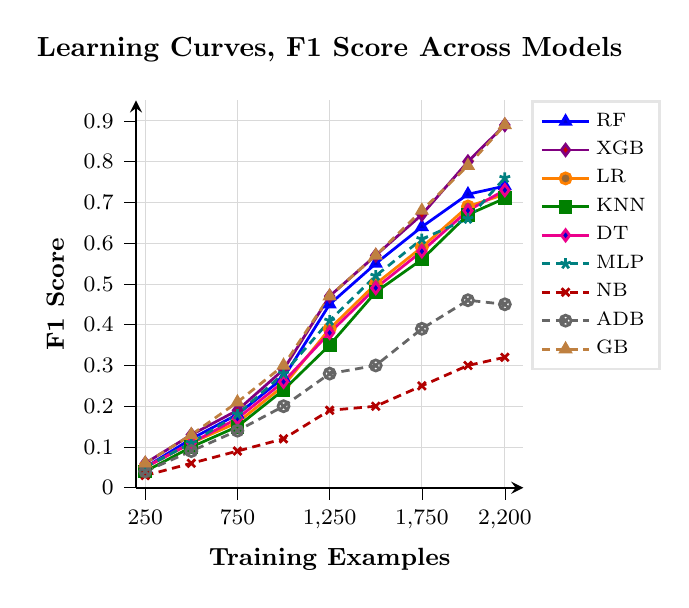
\begin{tikzpicture}
\begin{axis}[
    title={\textbf{Learning Curves, F1 Score Across Models}},
    title style={yshift=1.0ex},
    width=6.5cm, height=6.5cm,
    xlabel={\textbf{Training Examples}},
    ylabel={\textbf{F1 Score}},
    xmin=200, xmax=2300,
    ymin=0, ymax=0.95,
    xtick={250,750,1250,1750,2200},
    ytick={0,0.1,...,0.9},
    axis x line=bottom,
    axis y line=left,
    tick align=outside,
    tick style={black},
    grid=major,
    major grid style={line width=.3pt,draw=gray!30},
    tick label style={font=\footnotesize},
    label style={font=\small},
    scaled x ticks=false,
    scaled y ticks=false,
    x tick label style={/pgf/number format=fixed, /pgf/number format=1000 sep={,}},
    y tick label style={/pgf/number format=fixed, /pgf/number format=precision=1},
    legend style={
        at={(1.02,1)},        % original position
        anchor=north west,
        font=\scriptsize,
        draw=black!10, fill=white
    },
    legend cell align={left},
    legend image post style={scale=1.0},
    clip=false,
    line width=0.9pt
]

% Random Forest
\addplot+[mark=triangle*, color=blue, line width=1pt, mark size=2pt]
coordinates {(250,0.05) (500,0.12) (750,0.18) (1000,0.27) (1250,0.45) (1500,0.55) (1750,0.64) (2000,0.72) (2200,0.74)};
\addlegendentry{RF}

% XGBoost
\addplot+[mark=diamond*, color=violet, line width=1pt, mark size=2pt]
coordinates {(250,0.06) (500,0.13) (750,0.19) (1000,0.29) (1250,0.47) (1500,0.57) (1750,0.67) (2000,0.80) (2200,0.89)};
\addlegendentry{XGB}

% Logistic Regression
\addplot+[mark=*, color=orange, line width=1pt, mark size=2pt]
coordinates {(250,0.05) (500,0.11) (750,0.16) (1000,0.25) (1250,0.39) (1500,0.50) (1750,0.59) (2000,0.69) (2200,0.72)};
\addlegendentry{LR}

% KNN
\addplot+[mark=square*, color=green!50!black, line width=1pt, mark size=2pt]
coordinates {(250,0.04) (500,0.10) (750,0.15) (1000,0.24) (1250,0.35) (1500,0.48) (1750,0.56) (2000,0.67) (2200,0.71)};
\addlegendentry{KNN}

% Decision Tree
\addplot+[mark=diamond*, color=magenta, line width=1pt, mark size=2pt]
coordinates {(250,0.05) (500,0.11) (750,0.17) (1000,0.26) (1250,0.38) (1500,0.49) (1750,0.58) (2000,0.68) (2200,0.73)};
\addlegendentry{DT}

% MLP
\addplot+[mark=star, color=teal, line width=1pt, mark size=2pt]
coordinates {(250,0.05) (500,0.11) (750,0.18) (1000,0.28) (1250,0.41) (1500,0.52) (1750,0.61) (2000,0.66) (2200,0.76)};
\addlegendentry{MLP}

% Naive Bayes
\addplot+[mark=x, color=red!70!black, line width=1pt, mark size=2pt]
coordinates {(250,0.03) (500,0.06) (750,0.09) (1000,0.12) (1250,0.19) (1500,0.20) (1750,0.25) (2000,0.30) (2200,0.32)};
\addlegendentry{NB}

% AdaBoost
\addplot+[mark=otimes, color=gray!80!black, line width=1pt, mark size=2pt]
coordinates {(250,0.04) (500,0.09) (750,0.14) (1000,0.20) (1250,0.28) (1500,0.30) (1750,0.39) (2000,0.46) (2200,0.45)};
\addlegendentry{ADB}

% Gradient Boosting
\addplot+[mark=triangle*, color=brown, line width=1pt, mark size=2pt]
coordinates {(250,0.06) (500,0.13) (750,0.21) (1000,0.30) (1250,0.47) (1500,0.57) (1750,0.68) (2000,0.79) (2200,0.89)};
\addlegendentry{GB}

\end{axis}
\end{tikzpicture}
\caption{\textbf{Effect of Training Sample Size on F1 Score for Multiple Models in Tuple Classification (POB Task).} XGBoost and Gradient Boosting lead performance, especially as data volume increases.}
\label{fig:samplesVModels}
\end{figure}


Then, we used our best-performing model to evaluate its performance in each metric across different sample sizes. We can see from Fig. \ref{fig:samplesVsMetrics} a linear increase in precision, recall, and F1-score values as the number of samples grows. The accuracy values are the same as the recall values; hence, they're not shown on this graph.
\begin{figure}[!ht]
\centering
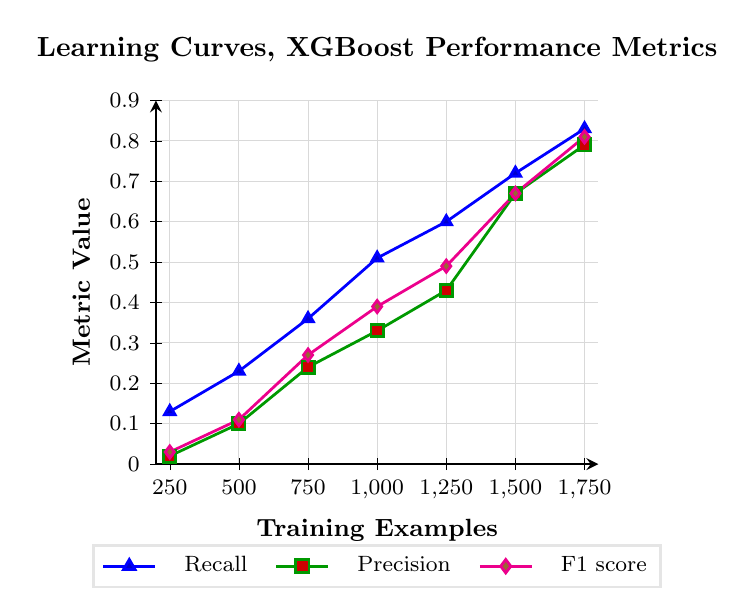
\begin{tikzpicture}
\begin{axis}[
    title={\textbf{Learning Curves, XGBoost Performance Metrics}},
    title style={yshift=1.0ex},
    width=7.2cm, height=6.2cm,
    xlabel={\textbf{Training Examples}},
    ylabel={\textbf{Metric Value}},
    xmin=200, xmax=1800,
    ymin=0, ymax=0.9,
    xtick={250, 500, 750, 1000, 1250, 1500, 1750},
    ytick={0,0.1,0.2,0.3,0.4,0.5,0.6,0.7,0.8,0.9},
    tick align=outside,
    tick style={black},
    axis x line=bottom,
    axis y line=left,
    major grid style={line width=.3pt, draw=gray!30},
    minor grid style={line width=.2pt, draw=gray!15},
    grid=major,
    tick label style={font=\footnotesize},
    label style={font=\small},
    scaled x ticks=false,
    scaled y ticks=false,
    y tick label style={/pgf/number format=fixed, /pgf/number format=precision=1},
    x tick label style={/pgf/number format=fixed, /pgf/number format=1000 sep={,}},
    legend style={
        at={(0.5,-0.22)},
        anchor=north,
        font=\footnotesize,
        legend columns=3,
        column sep=8pt,
        draw=black!10, fill=white,
    },
    legend image post style={scale=1.1},
    legend cell align={left},
    clip=false,
    line width=0.9pt
]

% Recall
\addplot+[mark=triangle*, color=blue, line width=1pt, mark size=2.2pt]
coordinates {(250,0.13) (500,0.23) (750,0.36) (1000,0.51) (1250,0.60) (1500,0.72) (1750,0.83)};
\addlegendentry{Recall}

% Precision
\addplot+[mark=square*, color=green!60!black, line width=1pt, mark size=2.2pt]
coordinates {(250,0.02) (500,0.10) (750,0.24) (1000,0.33) (1250,0.43) (1500,0.67) (1750,0.79)};
\addlegendentry{Precision}

% F1 score
\addplot+[mark=diamond*, color=magenta, line width=1pt, mark size=2.2pt]
coordinates {(250,0.03) (500,0.11) (750,0.27) (1000,0.39) (1250,0.49) (1500,0.67) (1750,0.81)};
\addlegendentry{F1 score}

\end{axis}
\end{tikzpicture}
\caption{\textbf{Effect of Training Sample Size on XGBoost Performance Metrics.} All metrics rise with sample size, with F1 score near 0.8 by 1750 examples.}
\label{fig:samplesVsMetrics}
\end{figure}

Next, we examine how the number of packets within a flow influences model accuracy for classifying the tuple (browser, OS, PQC). As illustrated in Fig.~\ref{fig:pacVModel} , the top-performing models already yield strong results after the first 10 packets, a pattern closely linked to the handshake, which is where the KEM effect on the traffic manifests. 

\begin{figure}[!ht]
\centering
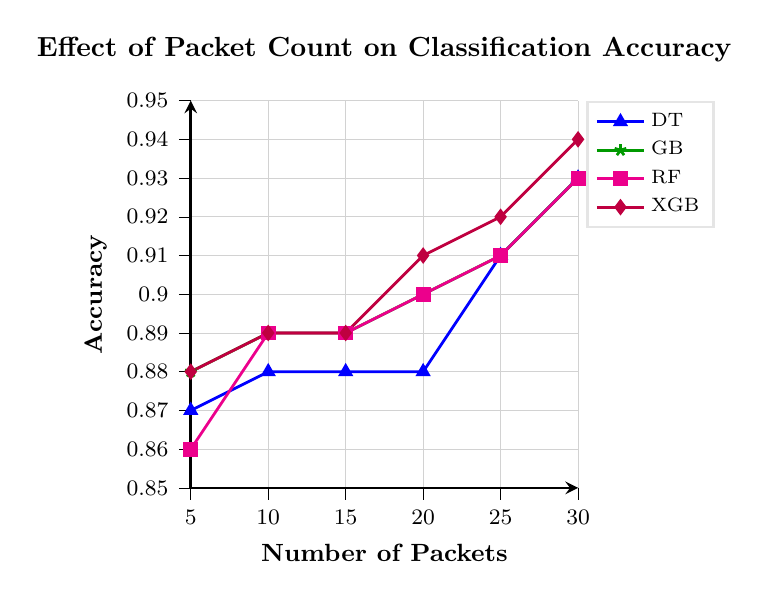
\begin{tikzpicture}
\begin{axis}[
    title={\textbf{Effect of Packet Count on Classification Accuracy}},
    title style={yshift=1.0ex},
    xlabel={\textbf{Number of Packets}},
    ylabel={\textbf{Accuracy}},
    xmin=5, xmax=30,
    ymin=0.85, ymax=0.95,
    width=6.5cm, height=6.5cm,
    xtick={5, 10, 15, 20, 25, 30},
    %ytick={0.3, 0.4, 0.5, 0.6, 0.7, 0.8, 0.85, 0.9, 0.95, 1.0},
    ytick={0.85,0.86,...,0.95},
    axis x line=bottom,
    axis y line=left,
    tick align=outside,
    tick style={black},
    grid=major,
    major grid style={line width=.3pt,draw=gray!35},
    minor grid style={line width=.2pt,draw=gray!20},
    tick label style={font=\footnotesize},
    label style={font=\small},
    legend style={
        at={(1.02,1)},
        anchor=north west,
        font=\scriptsize,
        draw=black!10, fill=white
    },
    legend cell align={left},
    legend image post style={scale=1.0},
    line width=1pt
]

% Decision Tree
\addplot+[color=blue, mark=triangle*, mark options={fill=blue}, mark size=2.2pt]
    coordinates {(5, 0.87) (10, 0.88) (15, 0.88) (20, 0.88) (25, 0.91) (30, 0.93)};
\addlegendentry{DT}

% Gradient Boosting
\addplot+[color=green!60!black, mark=star, mark options={fill=green!60!black}, mark size=2.2pt]
    coordinates {(5, 0.88) (10, 0.89) (15, 0.89) (20, 0.90) (25, 0.91) (30, 0.93)};
\addlegendentry{GB}

% Random Forest
\addplot+[color=magenta, mark=square*, mark options={fill=magenta}, mark size=2.2pt]
    coordinates {(5, 0.86) (10, 0.89) (15, 0.89) (20, 0.90) (25, 0.91) (30, 0.93)};
\addlegendentry{RF}

% XGBoost
\addplot+[color=purple, mark=diamond*, mark options={fill=purple}, mark size=2.2pt]
    coordinates {(5, 0.88) (10, 0.89) (15, 0.89) (20, 0.91) (25, 0.92) (30, 0.94)};
\addlegendentry{XGB}

\end{axis}
\end{tikzpicture}
\caption{\textbf{Effect of Packet Count on Classification Accuracy for Tuple-Level Prediction in the POB Task.} All models quickly approach high accuracy, with XGBoost achieving the highest score at 30 packets.}
\label{fig:pacVModel}
\end{figure}



Then, we used our best-performing model (XGBoost) to see the impact of packet increment on its performance using several different metrics. From Fig.~\ref{fig:pacVMetric} we can see that, similarly to Fig.~\ref{fig:pacVModel}, 10 packets deliver strong results yet again.
This strongly correlates with current studies such as Pesek et al.~\cite{11096965}, demonstrating strong classification results using only the first 10 packets of each flow as samples and TDL as their features.



% \begin{figure*}[!]
%     \centering
%     \footnotesize
%     \begin{tikzpicture}
%         \begin{axis}[
%             scaled y ticks = false,
%             ybar,
%             ymin=0, ymax=0.3,
%             bar width=0.5cm,
%             width= 14cm, height=3cm,
%             symbolic x coords={Packet 4 Length, Packet 1 Length, Packet 5 Length, Packet 12 Length, Packet 8 Length},
%             xtick=data,
%             xticklabel style={anchor=center, yshift=-1.5ex},
%             xlabel={},
%             ylabel={Importance},
%             axis lines=left,
%             nodes near coords,
%             nodes near coords style={
%                 /pgf/number format/fixed,
%                 /pgf/number format/precision=2
%             },
%             enlarge x limits=0.15,
%             ytick={0, 0.15, 0.3},
%             xticklabel style={/pgf/number format/precision=3,
%             /pgf/number format/fixed},
%             every tick/.style={draw=none},
%         ]
%             \addplot coordinates {(Packet 4 Length, 0.28) (Packet 1 Length, 0.20) (Packet 5 Length, 0.09) (Packet 12 Length, 0.06) (Packet 8 Length, 0.04)};
%         \end{axis}
%     \end{tikzpicture}
%     \caption{Summary of Feature Importance values for Decision Tree in POB classification task}
%     \label{fig:feature_importance}
% \end{figure*}


% \begin{figure*}
%     \centering
%     \footnotesize
%     \begin{tikzpicture}
%         \begin{axis}[
%             ybar,
%             ymin=0.75, ymax=1,
%             bar width=0.5cm,
%             width= 14cm, height=3cm,
%             symbolic x coords={PQC/No-PQC, Browser classification, OS classification, PQC Browser OS, PQC more packets},
%             xtick=data,
%             xticklabel style={anchor=center, yshift=-1.5ex}, % Center the x-labels under the bars
%             xlabel={},
%             ylabel={Accuracy},
%             axis lines=left,
%             nodes near coords,
%             enlarge x limits=0.15,
%             ytick={0, 0.2, 0.4, 0.6, 0.8, 1},
%             every tick/.style={draw=none},
%         ]
%             \addplot coordinates {(PQC/No-PQC, 0.93) (Browser classification, 0.95) (OS classification, 0.99) (PQC Browser OS, 0.91) (PQC more packets, 0.96)};
%         \end{axis}
%     \end{tikzpicture}
%     \caption{Summary of Accuracy Results for All Experiments in POB classification task}
%     \label{fig:accuracy_experiments}
% \end{figure*}




We also examined the feature importance of our model. From Fig.~\ref{fig:feature_importance}, we see that the most important feature is the length of the 4$^{th}$ packet. Upon inspecting our data, we see that the fourth packet is the TLS ClientHello packet, in which the PQC algorithm chosen manifests as a part of the "supported groups" and "signature algorithms" fields. The second most important feature is the length of the first packet - the SYN.
\begin{figure}[htbp]
\centering
\footnotesize
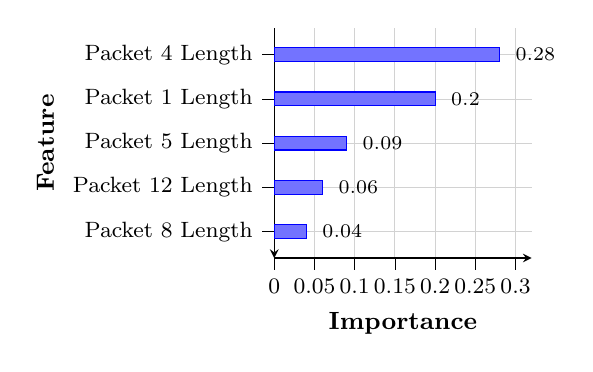
\begin{tikzpicture}
\begin{axis}[
    xbar,
    xmin=0, xmax=0.32,
    width=0.4\textwidth, height=4.5cm,
    bar width=5pt,
    symbolic y coords={{Packet 4 Length},{Packet 1 Length},{Packet 5 Length},{Packet 12 Length},{Packet 8 Length}},
    ytick=data,
    y dir=reverse,
    xlabel={\textbf{Importance}},
    ylabel={\textbf{Feature}},
    xtick={0,0.05,0.10,0.15,0.20,0.25,0.30},
    xticklabel style={/pgf/number format/fixed, /pgf/number format/precision=2},
    axis x line=bottom,
    axis y line=left,
    tick align=outside,
    tick style={black},
    grid=major,
    major grid style={line width=.3pt,draw=gray!35},
    enlarge y limits=0.15,
    tick label style={font=\footnotesize},
    label style={font=\small},
    % show values outside the bars
    nodes near coords={\pgfmathprintnumber[fixed,precision=2]{\pgfplotspointmeta}},
    nodes near coords style={font=\scriptsize\bfseries, anchor=west, xshift=0.8mm, text=black},
    nodes near coords align={west},
    point meta=x
]

\addplot+[fill=blue!55, draw=blue] coordinates
  {(0.28,{Packet 4 Length})
   (0.20,{Packet 1 Length})
   (0.09,{Packet 5 Length})
   (0.06,{Packet 12 Length})
   (0.04,{Packet 8 Length})};

\end{axis}
\end{tikzpicture}
\caption{Feature importance for the Decision Tree in the POB classification task, sorted by descending contribution.}
\label{fig:feature_importance}
\end{figure}

In all experiments for the PQC-POB classification tasks, we have seen that XGBoost achieves the best results in each experiment. We also observed that the Random Forest model consistently delivers strong results. All best results for each classification task can be inferred from Fig.~\ref{fig:accuracy_experiments}.
\begin{figure}[htbp]
\centering
\footnotesize
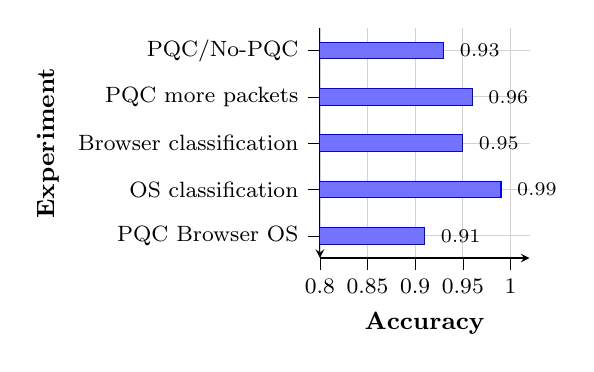
\begin{tikzpicture}
\begin{axis}[
    xbar,
    xmin=0.8, xmax=1.02,
    width=0.35\textwidth, height=4.5cm,
    bar width=6pt,
    symbolic y coords={PQC/No-PQC, PQC more packets, Browser classification, OS classification, PQC Browser OS},
    ytick=data,
    y dir=reverse,
    xlabel={\textbf{Accuracy}},
    ylabel={\textbf{Experiment}},
    xtick={0.75,0.80,0.85,0.90,0.95,1.00},
    axis x line=bottom,
    axis y line=left,
    tick align=outside,
    tick style={black},
    grid=major,
    major grid style={line width=.3pt,draw=gray!35},
    enlarge y limits=0.12,
    tick label style={font=\footnotesize},
    label style={font=\small},
    nodes near coords={\pgfmathprintnumber[fixed,precision=2]{\pgfplotspointmeta}},
    nodes near coords align={west},
    nodes near coords style={font=\scriptsize, anchor=west, xshift=0.8mm, text=black},
    point meta=x
]
\addplot+[fill=blue!55, draw=blue] coordinates
  { (0.93,{PQC/No-PQC})
    (0.96,{PQC more packets})
    (0.95,{Browser classification})
    (0.99,{OS classification})
    (0.91,{PQC Browser OS})};
\end{axis}
\end{tikzpicture}
\caption{Summary of accuracy across experiments for the POB classification task.}
\label{fig:accuracy_experiments}
\end{figure}


\section{PQC-Algo Experimental Results}
\label{sec:algoex}
In this section, we use the PQC-Algo dataset, explicitly crafted for this classification task, which contains traffic of the two types of PQC algorithms, ML-KEM and Kyber\cite{NIST_FIPS_203_2024}. We analyze the subtle classification distinctions between the two types of algorithms while using PQC encryption.
The objective was to determine whether delicate yet essential traffic data could be accurately classified due to the constant advancements in the PQC realm.


\subsection{PQC Algorithm classification}
In this experiment, we evaluate the ability of machine learning models to distinguish between different PQC algorithms (ML-KEM and Kyber) based solely on encrypted traffic patterns. Table \ref{tab:algorithms} presents the results for classifying different PQC algorithms. According to the table, the Ensemble Boosting models (e.g., AdaBoost, Gradient Boosting and XGBoost) outperform other classifiers, achieving the highest accuracy and AUC.


\subsection{Algorithm, Browser (Tuple) classification}
The classification results for a combination of each browser (Chrome, Firefox) with each PQC algorithm (ML-KEM, Kyber) are shown in Table \ref{tab:tuple}. This experiment aimed to identify behavioral differences in real-life scenarios. The Random Forest model achieves the highest accuracy and the best AUC.  


Similar to the previous POB classification results, XGBoost delivers the best classification results for each experiment yet again.

\section{Discussion and Conclusions}
\label{sec:disc}
We introduce two key innovations in classifying whether the user uses PQC and user environments. First, our research leverages actual encrypted traffic that uses PQC for classification, a departure from the common practice of simulating network behaviors. This approach provides more accurate and realistic insights into the performance of PQC protocols in real-world scenarios, thereby enhancing the reliability and applicability of our classification models. Second, we have developed a model that distinguishes between PQC and No-PQC algorithms, adding a critical layer of specificity to the classification process. With the assistance of a PQC algorithm, we demonstrate that both the browser and the operating system used by the user can be accurately identified.
The results provided in Sections~\ref{sec:pobex} and \ref{sec:algoex} set the first benchmark for accurately classifying traffic encrypted with PQC under various scenarios. As can be inferred from Tables ~\ref{tab:pqcVsnpqc} - ~\ref{tab:all}, the XGBoost and Random Forest classifiers consistently deliver strong performance, particularly when tackling complex classification tasks that involve multiple parameters.
This research is significant because it has the potential to enhance the security and efficiency of Internet communications in the era of quantum computing. As quantum computers advance, traditional cryptographic methods face the threat of becoming obsolete. Our research addresses this by classifying encrypted traffic that uses PQC, which is designed to be secure against quantum attacks. Accurately classifying these algorithms is crucial for identifying vulnerabilities and ensuring robust security measures. In addition, by analyzing the effects of browsers used by the user on the identity of the PQC algorithm, critical aspects of user privacy and service optimization further contribute to the security and efficiency of Internet communications. This paper’s findings are based on PQC traffic recorded in various network settings. 
As PQC traffic becomes more prevalent, our analysis of real-world (“in the wild”) traffic is crucial. In this research, we're leveraging a broader dataset in addition to classifying PQC traffic as a whole and distinguishing specific NIST algorithms within these different environments. Such granularity allows us to deepen our understanding of PQC performance in diverse environments and foster the development of comprehensive security solutions tailored for the post-quantum era.
Future research could expand this work by leveraging a broader dataset drawn from widely used applications, such as Zoom~\cite{zoom2024postquantum} and other PQC-utilizing applications. In addition, the ability of the framework to identify the algorithm and OS will set the basis for our ability to investigate the possibility of PQC crypto agility. Based on our results, we aim to determine that the OS of a certain machine has limited computational capabilities and can delegate tasks to another device.

\begin{table}
\centering
\caption{Algorithm Classification Results}
\vspace{1.5mm}
\label{tab:algorithms}
\begin{tabular}{|l|l|l|l|l|l|}
\hline
Model               & Acc & Pre & Rec & F1 & AUC  \\ \hline\hline
ADB            & 0.66     & 0.66      & 0.66   & 0.62     & 0.85 \\ \hline
DT       & 0.78     & 0.79      & 0.79   & 0.78     & 0.85 \\ \hline
GB   & 0.78     & 0.78      & 0.78   & 0.78     & 0.88 \\ \hline
KNN                 & 0.74     & 0.75      & 0.74   & 0.74     & 0.86 \\ \hline
LR & 0.72     & 0.73      & 0.72   & 0.72     & 0.85 \\ \hline
MLP                 & 0.74     & 0.74      & 0.73   & 0.71     & 0.84 \\ \hline
NB         & 0.74     & 0.78      & 0.74   & 0.69     & 0.85 \\ \hline
RF       & 0.78     & 0.77      & 0.78   & 0.78     & 0.88 \\ \hline
XGB             & 0.78     & 0.78      & 0.78   & 0.78     & 0.88 \\ \hline
\end{tabular}
\end{table}



\begin{table}[!]
\centering
\caption{Classify Tuple: Browser and Algorithm (Kyber, ML-KEM)}
\vspace{1.5mm}
\label{tab:tuple}
\begin{tabular}{|l|l|l|l|l|l|}
\hline
Model               & Acc & Pre & Rec & F1 & AUC  \\ \hline \hline
AdaBoost            & 0.55     & 0.53      & 0.55   & 0.46     & 0.81 \\ \hline
DT       & 0.72     & 0.73      & 0.73   & 0.73     & 0.82 \\ \hline
GB   & 0.76     & 0.76      & 0.76   & 0.76     & 0.92 \\ \hline
KNN                 & 0.67     & 0.68      & 0.67   & 0.67     & 0.88 \\ \hline
LR & 0.66     & 0.65      & 0.66   & 0.65     & 0.88 \\ \hline
MLP                 & 0.69     & 0.68      & 0.69   & 0.65     & 0.87 \\ \hline
NB         & 0.63     & 0.62      & 0.63   & 0.57     & 0.83 \\ \hline
RF      & 0.75     & 0.75      & 0.74   & 0.75     & 0.92 \\ \hline
XGB             & 0.76     & 0.76      & 0.76   & 0.76     & 0.92 \\ \hline
\end{tabular}
\end{table}


\section{Acknowledgments}
This research was supported by the Ministry of Innovation, Science \& Technology, Israel. The EU Horizon COCOON Project supported this work under Grant Agreement No 101120221.

\bibliographystyle{ieeetr}
\bibliography{bib}

\end{document}


